\documentclass{beamer}
\usepackage[utf8]{inputenc}
\usepackage{amsfonts,url}
\usepackage{amsmath}
\usepackage{mathtools}
\usepackage{amssymb}
\usepackage{xcolor}
\usepackage{verbatim}
\usepackage{tikz}
\usepackage{wrapfig}
\usepackage{lipsum}
\usetikzlibrary{svg.path, automata, positioning, arrows, shapes,snakes, matrix}
\usepackage{amssymb}
%regarding include graphics
\usepackage{graphicx}
\graphicspath{ {./images/} }
\usepackage{float}


\usetheme{default}
\usecolortheme{beaver}


% Use the following symbols for number sets
\newcommand{\R}{\mathbb R}
\newcommand{\N}{\mathbb N}
\newcommand{\Z}{\mathbb Z}
\newcommand{\C}{\mathbb C}
\newcommand{\Q}{\mathbb Q}




%%°°°°°°°°°°°°°°°°°°°°COMMANDS°°°°°°°°°°°°°°°°°°°°
%my Special emphatic commands:
\newcommand{\obs}{}				%for text aimed at observing something
\newcommand{\word}{\mathbf}				%used for variables who represent a word
\newcommand{\mtxt}{\textrm}				%used for text in mathematical definitions
\newcommand{\abece}{\mathbf{X}}			%alphabeth
\newcommand{\fslovar}{\mathbf{X^*}}		%dictionary
\newcommand{\infslovar}{\mathbf{X^\omega}}		%infinite dictionary
\newcommand{\auto}{\mathcal}			%usual for automata
\newcommand{\QQ}{\mathcal{Q}}			%set of States 
\newcommand{\prefix}{\mathcal{P}}	%to sign the prefix of a set ofwords
\newcommand{\semisynaut}{\mathcal{FSA}}	%set of synchronous automatic, NOT invertible
\newcommand{\synaut}{\mathcal{GA}}	%set of synchronous automatic functions, invertible
\newcommand{\PI}{\bar{\pi}}			%to write the pi expansion
\newcommand{\LAMBDA}{\bar{\lambda}}			%to write the lambda expansion
\newcommand{\LL}{\mathcal{L}}		%lamplighter group

\DeclareMathOperator{\aut}{\mathcal{AUT}}		%set of some automorphisms on a set
\DeclareMathOperator{\symm}{\mathcal{S}}		%simmetric group, the group of permutations
\DeclareMathOperator{\id}{\mathrm{id}}			%identityt element





\title{Groups of  Automata}
\author{Carlo Lanzi Luciani}
\institute{Mentors:\\ izr. prof. Ganna Kudryavtseva\\ prof. Alessandro Logar}
\date{\today}
\logo{
\includegraphics[scale=0.04]{Images/units.jpeg} 
\includegraphics[scale=0.3]{Images/univerza v ljubljani.png} 
}

\begin{document}


%1title frame
\begin{frame}
  \titlepage{}
\end{frame}



%\begin{figure}[!h]
%\begin{tikzpicture}[scale=0.8, every node/.style={transform shape}]
%\node (aut) at (0,-4 cm) {Automaton $\auto{A}$};
%
%\node  [draw=black, align=center, minimum width=2.5cm, minimum height=1.5cm, xshift=5cm] (init aut) at (aut) {Initial\\ automaton $\auto{A}_{q_0}$};
%
%\draw  (aut) edge[dashed,below,->] node[scale=0.8,transform shape]{defines} (init aut);
%
%\node  [yshift=1.5cm] (input) at (init aut){};
%
%\node  [right, color=blue] at (input) {input};
%
%\node  [yshift=-1.5cm] (output) at (init aut){};
%\node  [right, color=violet] at (output) {output};
%
%\path  [draw, line width=0.5mm, color=blue,->] (input)->(init aut);
%\path  [draw, line width=0.5mm, color=violet,->] (init aut)->(output);
%
%\node [align=center, xshift=5cm] (action) at (init aut) {Action\\ $f(\text{input})=\text{output}$};
%\draw (init aut) edge[dashed,below,->] node[scale=0.8,transform shape] {defines} (action);
%\node [state, xshift=2cm,yshift=-2cm] (aim) at (action) {My aim};
%\draw (aim) edge[bend left,->] (action);
%\end{tikzpicture}
%\end{figure}



%1intention's declaration
\begin{frame}
\frametitle{1. Introduction}
The word \alert{automaton}: from the greek "acting of one's own will". Automat\alert{a} are important in:
\begin{itemize}
\item Information theory
\item Theory of dynamical systems
\item Algebra
\item Others
\end{itemize}

My aim: study some of the groups constructed through a special class of them, the invertible deterministic Mealy automata, here called simply automata.
\begin{figure}[h]
\centering
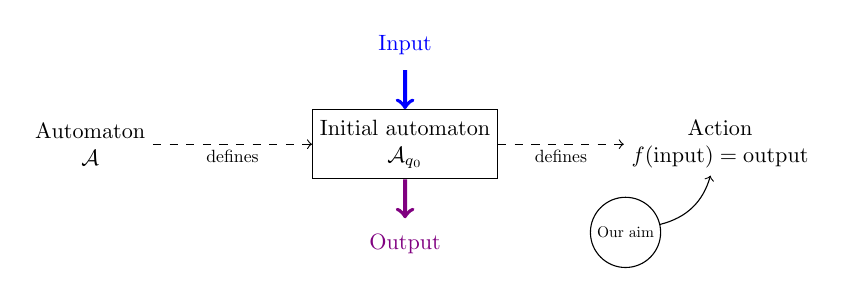
\begin{tikzpicture}[scale=0.8, every node/.style={transform shape}]

\node [draw=black,minimum width=2.5cm,minimum height=1.1cm,align=center](init aut) at (0,0) {Initial automaton\\ $\auto{A}_{q_0}$};

\node [xshift=-5cm,align=center](aut) at (init aut) {Automaton\\ $\auto{A}$};


\draw (aut) edge[dashed,below,->] node[scale=0.8,transform shape]{defines} (init aut);

\node  [yshift=1.3cm](input) at (init aut){};
\node  [above, color=blue] at (input) {Input};
\node  [yshift=-1.3cm](output) at (init aut){};
\node  [below, color=violet] at (output) {Output};
\path  [draw, line width=0.5mm, color=blue,->] (input)->(init aut);
\path  [draw, line width=0.5mm, color=violet,->] (init aut)->(output);

\node  [align=center,xshift=5cm](action) at (init aut) {Action\\ $f(\text{input})=\text{output}$};
\draw  (init aut) edge[dashed,below,->] node[scale=0.8,transform shape]{defines} (action);
\node  [state,xshift=3.5cm,yshift=-1.4cm,scale=0.7] (aim) at (init aut) {Our aim};
\draw  (aim) edge[bend right,->] (action);
\end{tikzpicture}
\end{figure}
\end{frame}


%2superbrief intro on word spaces
%\begin{frame}
%\frametitle{Alphabet and the Free Monoid}
%Let $\abece$ be finite set, called the \textit{Alphabet}. Then we have:
%\begin{itemize}
%\item $\fslovar=\{x_{1}x_{2}\ldots x_{n}:x_{i}\in X, n\in\N\cup\{0\}\}$ the \textit{Free Monoid}
%\item Composition of words: $\word{w}\circ\word{v}:=\word{w} \word{v}$\pause
%\item The Empty Word $\varnothing$\pause
%\item Lenght of words: if $\word{w}=x_1 \ldots x_n$ then $|\word{w}|:=n$
%\end{itemize}\pause


%\begin{example}
%Let $\abece=\{0,1\}$ and let $\word{w}=0010$ and $\word{v}=010$. Then $\word{w}\circ \word{v}=0010\circ010=0010010$, $|\word{w}|=4$ and $|\word{v}|=3$.
%\end{example}
%\end{frame}



%\begin{comment}
%\item Alphabet Tree:

%
%%picture of an  Automata
%\begin{frame}
%\frametitle{An Example with Moore diagrams}
%\begin{block}{Moore diagrams}
%We put $G=(\QQ,E)$ with $E:=\{(q_i,q_j)|\exists \word{w} \in X : \pi(\word{w},q_i)=q_j\}$
%\end{block}
%%Here instead of giving the exact definition of the extension I explain it through the graph
%\end{frame}
%
%\end{comment}



%introduction to Automata
\begin{frame}
\frametitle{2. The automaton}
\begin{block}{Definition}
An \alert{automaton} is a 4-tuple $\auto{A}=\langle\abece,\QQ,\pi,\lambda\rangle$ where:
\begin{itemize}
	\item $\abece=\{x_1,\:\ldots\:,x_k\}$ is a finite set called the \alert{alphabet},
	% so here we declare what we put inside and what comes aoutside of the machine
	\item $\QQ$ is a set called the \alert{set of internal states of the  automaton},
	\item $\pi:\textcolor{blue}{\abece}\times\QQ \longrightarrow \QQ $ is a function called the \alert{transition function},
	\item $\lambda:\textcolor{blue}{\abece}\times\QQ \longrightarrow \textcolor{violet}{\abece}$ is a function such that $\lambda_q=\lambda(\cdot,q):\abece\longrightarrow\abece$ is bijective, and is called the \alert{output function}.
\end{itemize}
\end{block}\pause
\begin{figure}[h!]
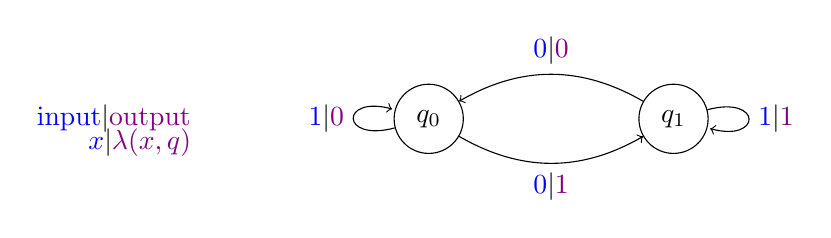
\begin{tikzpicture}
%\textcolor{violet}
%\textcolor{blue}
\node[state](q0) at (0,0) {$q_0$};
\node[state, right of=q0, xshift=60] (q1) {$q_1$};
\node [align=center] (text) at (-4cm,0) {$\textcolor{blue}{\text{input}}|\textcolor{violet}{\text{output}}$};
\node [align=center, below,xshift=0.33cm] at (text) {$\textcolor{blue}{x}|\textcolor{violet}{\lambda(x,q)}$};

\draw	(q0) edge[below,bend right,-> ] node{$\textcolor{blue}{0}|\textcolor{violet}{1}$} (q1)
		(q0) edge[loop left] node{$\textcolor{blue}{1}|\textcolor{violet}{0}$} (q0)
		(q1) edge[loop right] node{$\textcolor{blue}{1}|\textcolor{violet}{1}$} (q1)
		(q1) edge[above, bend right,-> ] node{$\textcolor{blue}{0}|\textcolor{violet}{0}$} (q0);
		
\end{tikzpicture}
%\onslide<5->
\caption{Moore diagram of a 2-state automaton over $\abece=\{0,1\}$}
\end{figure}
\end{frame}



\begin{frame}
\frametitle{3. The initial automaton}
\begin{block}{Definition}
$\fslovar=\{x_{1}x_{2}\ldots x_{n}:x_{i}\in X, n\in\N\cup\{0\}\}$ the \alert{dictionary}.

Word composition: $x_{1}\ldots x_{n}. z_{1}\ldots z_{n}:=x_{1}\ldots x_{n} z_{1}\ldots z_{n}$
\end{block}\pause
%\textcolor{violet}
%\textcolor{blue}
\begin{Definition}
An \alert{initial automaton $\auto{A}_{q_0}$} is an automaton $\auto{A}$ with a fixed state $q_0$. 
The \alert{action of $\auto{A}_{q_0}$} is the function $\LAMBDA_{q_0}:\fslovar\longrightarrow \fslovar$ with $\LAMBDA_{q_0}(\textcolor{blue}{x_1x_2\ldots x_n})=\textcolor{violet}{y_1y_2\ldots y_n}$.
\end{Definition}%\pause
\begin{figure}
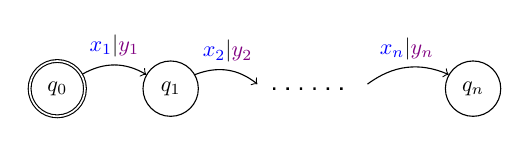
\begin{tikzpicture}[scale=0.8, every node/.style={transform shape}]
\node[state, accepting](q0) at (0,1cm) {$q_0$};
\node[state, right of=q0,xshift=0.8cm] (q1) {$q_1$};
\node[right of=q1,xshift=0.5cm] (qan1) {};
\node[right of=qan1,xshift=0.5cm] (qan2) {};
\node[state, right of=qan2,xshift=0.8cm] (qn) {$q_n$};

\draw	(q0) edge[above,bend left,-> ] node{$\textcolor{blue}{x_1}|\textcolor{violet}{y_1}$} (q1)
		(q1) edge[above,bend left,-> ] node{$\textcolor{blue}{x_2}|\textcolor{violet}{y_2}$} (qan1)
		(qan1) edge[line width=0.3mm, loosely dotted] (qan2)
		(qan2) edge[above,bend left,-> ] node{$\textcolor{blue}{x_n}|\textcolor{violet}{y_n}$} (qn);
\end{tikzpicture}
\end{figure}
\end{frame}




%\begin{frame}
%\frametitle{4. Composition of Initial automata}
%\begin{block}{Proposition}
%Given initial automata $(\auto{A}_1)_{q_1}$ and $(\auto{A}_2)_{q_2}$ with actions $\LAMBDA^{\auto{A}_1}_{q_1}$ and $\LAMBDA^{\auto{A}_2}_{q_2}$, there exists an initial automaton $\auto{B}_p$ with action $\LAMBDA^{\auto{B}}_p$ such that:
% $$\LAMBDA^{\auto{A}_2}_{q_2} \circ \LAMBDA^{\auto{A}_1}_{q_1}=\LAMBDA^{\auto{B}}_p.$$
%\end{block}
%\begin{figure}[H]
%\begin{tikzpicture}[scale=0.7,  every node/.style={transform shape}]
%\node[draw,rectangle,minimum width=1.25cm, minimum height = 1.25cm] (auto1) at (-3cm,0) {$(\auto{A}_1)_{q_1}$};
%\node (input) at (-6cm,0) {};
%\node[above, color=blue] at (input) {$\word{w}$};
%\node[draw,rectangle,minimum width=1.25cm, minimum height = 1.25cm] (auto2) at (3cm,0) {$(\auto{A}_2)_{q_2}$};
%\node (output) at (6cm,0) {};
%\node[above, color=violet] at (output) {$(\LAMBDA^{\auto{A}_2}_{q_2} \circ \LAMBDA^{\auto{A}_1}_{q_1})(\word{w})$};
%\node[draw,rectangle,minimum width=8cm, minimum height = 3cm] (auto1*auto2) at (0,0){};
%\node[above,color=purple] at (auto1*auto2) {$(\LAMBDA^{\auto{A}_1}_{q_1})(\word{w})$};
%\node at (0,2.1cm) {$ \auto{B}_p$};
%\draw (input) edge[line width=1.6pt,color=blue,->] (auto1);
%\draw (auto1) edge[line width=1.6pt,color=purple,->] (auto2);
%\draw (auto2) edge[line width=1.6pt,color=violet,->] (output);
%\end{tikzpicture}
%\end{figure}
%\end{frame}

%\begin{tikzpicture}[level distance=1cm,
%level 1/.style={sibling distance=5.5cm},
%level 2/.style={sibling distance=3.5cm, fontscale/.style = small},
%level 3/.style={sibling distance=0.8cm},
%level 4/.style={sibling distance=0.5cm}]
%
%\node{$\varnothing$} child[left] {node{0}child[right]{node{01} child[left]{node{010} child[dotted,line width=0.2mm] child[dotted,line width=0.2mm]} child[right]{node{011} child[dotted,line width=0.2mm] child[dotted,line width=0.2mm]}	} child[left]{node{00} child[left]{node{000}child[dotted,line width=0.2mm]child[dotted,line width=0.2mm]} child[right]{node{001}child[dotted,line width=0.2mm]child[dotted,line width=0.2mm]}	}	}  child[right] {node{1} child[right]{node{11} child[left]{node{110}child[dotted,line width=0.2mm]child[dotted,line width=0.2mm]} child[right]{node{111}child[dotted,line width=0.2mm]child[dotted,line width=0.2mm]}	} child[left]{node{10} child[left]{node{100}child[dotted,line width=0.2mm]child[dotted,line width=0.2mm]} child[right]{node{101}child[dotted,line width=0.2mm]child[dotted,line width=0.2mm]}	}	};
%\end{tikzpicture}





\begin{frame}
\frametitle{4. The word tree $\fslovar$}
\begin{block}{Definition}
Given $\word{w},\word{v}\in\fslovar$, $\word{w}$ is a child of $\word{v}$ if and only if $\word{w}=\word{v}.x=\word{v}x$ for some letter $x\in\abece$.
\end{block}
\begin{figure}
\centering
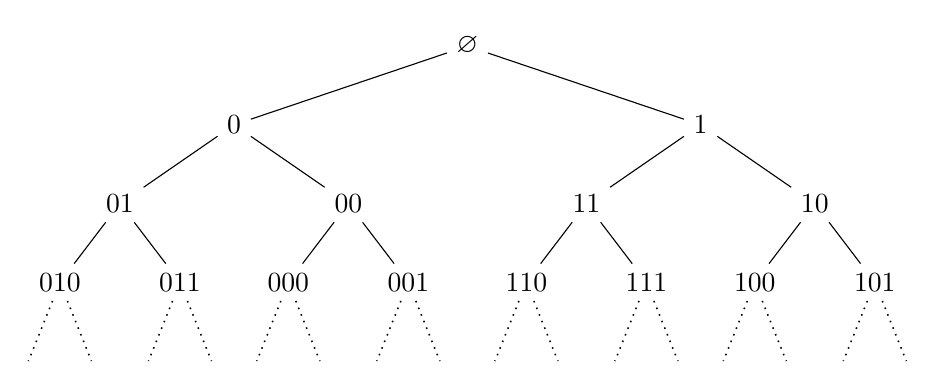
\begin{tikzpicture}[level distance=1cm,
level 1/.style={sibling distance=5.5cm},
level 2/.style={sibling distance=3.5cm, fontscale/.style = small},
level 3/.style={sibling distance=2.3cm},
level 4/.style={sibling distance=0.8cm}]

\node{$\varnothing$} child[left] {node{0}child[right]{node{01} child[right]{node{010} child[dotted,line width=0.2mm] child[dotted,line width=0.2mm]} child[left]{node{011} child[dotted,line width=0.2mm] child[dotted,line width=0.2mm]}	}
child[left]{node{00} child[right]{node{000}child[dotted,line width=0.2mm]child[dotted,line width=0.2mm]} child[left]{node{001}child[dotted,line width=0.2mm]child[dotted,line width=0.2mm]}	}	}
                	child[right] {node{1} child[right]{node{11} child[right]{node{110}child[dotted,line width=0.2mm]child[dotted,line width=0.2mm]} child[left]{node{111}child[dotted,line width=0.2mm]child[dotted,line width=0.2mm]}	} child[left]{node{10} child[right]{node{100}child[dotted,line width=0.2mm]child[dotted,line width=0.2mm]} child[left]{node{101}child[dotted,line width=0.2mm]child[dotted,line width=0.2mm]}	}	};
\end{tikzpicture}
\caption{An example of the word tree $\fslovar$ on $\abece=\{0,1\}$.}
\end{figure}
\end{frame}


\begin{frame}
\frametitle{5. Actions as tree-automorphisms}
\begin{block}{Proposition}
A function $f:\fslovar\longrightarrow\fslovar$ is the action of some initial automaton if and only if is a \alert{tree-automorphism} on the word tree $\fslovar$, i.e.:
\begin{itemize}
\item $f(\varnothing)=\varnothing$.
\item if $\word{w}\in\fslovar$ is a child of $\word{v}$ then $f(\word{w})$ is a child of $f(\word{v})$.
\item f is bijective.
\end{itemize}
\end{block}
\begin{figure}
%\begin{wrapfigure}{r}{3cm}
\centering
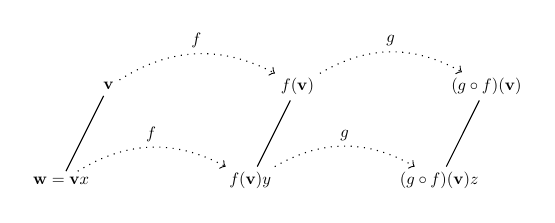
\begin{tikzpicture}[scale=0.6,every node/.style={transform shape}]
\node(v) at (0,2cm) {$\word{v}$};
\node(w)[xshift=-1cm,yshift=-2cm] at (v) {$\word{w}=\word{v}x$};

\node(fv)[xshift=4cm] at (v) {$f(\word{v})$};
\node(fw)[xshift=-1cm,yshift=-2cm] at (fv) {$f(\word{v})y$};

\node(gv)[xshift=4cm] at (fv) {$(g\circ f)(\word{v})$};
\node(gw)[xshift=-1cm,yshift=-2cm] at (gv) {$(g\circ f)(\word{v})z$};

\draw	(v) edge node(mid){} (w)
		(fv) edge node(fmid){} (fw)
		(v) edge[bend left, dotted,->]node[above] {$f$} (fv)
		(w) edge[bend left, dotted,->]node[above] {$f$} (fw);		
\draw	(gv) edge node(mid){} (gw)
		(fv) edge[bend left, dotted,->]node[above] {$g$} (gv)
		(fw) edge[bend left, dotted,->]node[above] {$g$} (gw);
\end{tikzpicture}
\end{figure}
%\end{wrapfigure}
\begin{block}{Proposition}
If $f,g$ are tree-automorphisms on $\fslovar$, then $g\circ f$ and $f^{-1}$ are tree-automorphisms on $\fslovar$.
\end{block}
\end{frame}


%\item Let $\auto{A}$ be a Synchronous  Automaton with its action $f$. It's invertible \textbf{(exists $\auto{A}'$ with its action $f'$ such that $f\circ f'=id$)} \emph{if and only if} $\lambda(\cdot,q) $ is invertible 
%(Memento: $\lambda(\cdot ,q) $ is exactly the action of the  Automaton)
%$$x|y\longrightarrow y|x$$

\begin{frame}
\frametitle{6. Groups defined by automata}
\begin{block}{Proposition}
The functions $f:\fslovar\longrightarrow \fslovar$ defined by initial automata (i.e. tree-automorphisms), called \alert{synchronous automatic permutations}, form a group denoted by $\aut_{tree}(\fslovar)$.
\end{block}\pause
\begin{Definition}
Let $\auto{A}=\langle \abece,\QQ,\pi,\lambda\rangle$ be an automaton. The \alert{group defined by $\auto{A}$} is the group generated by the set $\{\LAMBDA_q:q\in\QQ\}$.
\end{Definition}

\begin{figure}[h]
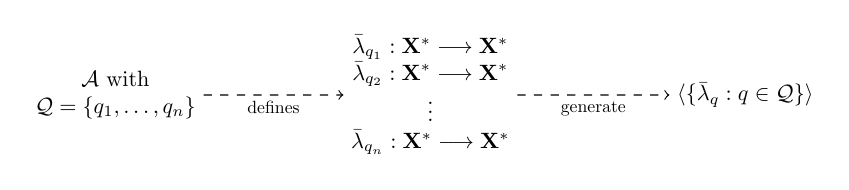
\begin{tikzpicture}[scale=0.8, every node/.style={transform shape}]
\node [align=center] (aut) at (0,-5 cm) {$\auto{A}$ with\\ $\QQ=\{q_1,\ldots,q_n\}$};

\node  [align=center,xshift=5cm] (actions) at (aut) {$\LAMBDA_{q_1}:\fslovar\longrightarrow\fslovar$\\ $\LAMBDA_{q_2}:\fslovar\longrightarrow\fslovar$\\ $\vdots$\\ $\LAMBDA_{q_n}:\fslovar\longrightarrow\fslovar$};

\draw  (aut) edge[dashed,below,->] node[scale=0.8,transform shape]{defines} (actions);

\node [align=center, xshift=5cm] (group) at (actions) {$\langle\{\LAMBDA_q:q\in\QQ\}\rangle$};
\draw (actions) edge[dashed,below,->] node[scale=0.8,transform shape] {generate} (group);
\end{tikzpicture}
\end{figure}
\end{frame}





%\raggedleft
%\begin{tikzpicture}[level distance=1cm,
%level 1/.style={sibling distance=5.5cm},
%level 2/.style={sibling distance=3.5cm, fontscale/.style = small},
%level 3/.style={sibling distance=2cm},
%level 4/.style={sibling distance=0.8cm}, every node/.style={transform shape},xscale=0.5,yscale=0.8]
%
%\node{$\varnothing$} child[left] {node(0){0}child[right]{node{01} child[right]{node{010} child[dotted,line width=0.2mm] child[dotted,line width=0.2mm]} child[left]{node{011} child[dotted,line width=0.2mm] child[dotted,line width=0.2mm]}	}
%child[left]{node{00} child[right]{node{000}child[dotted,line width=0.2mm]child[dotted,line width=0.2mm]} child[left]{node{001}child[dotted,line width=0.2mm]child[dotted,line width=0.2mm]}	}	}
%                	child[right] {node(1){1} child[right]{node{11} child[right]{node{110}child[dotted,line width=0.2mm]child[dotted,line width=0.2mm]} child[left]{node{111}child[dotted,line width=0.2mm]child[dotted,line width=0.2mm]}	} child[left]{node{10} child[right]{node{100}child[dotted,line width=0.2mm]child[dotted,line width=0.2mm]} child[left]{node{101}child[dotted,line width=0.2mm]child[dotted,line width=0.2mm]}	}	};
%\end{tikzpicture}

% $\varphi(\alpha)((f_{x_1}, \ldots ,f_{x_k}))=(f_{\alpha(x_1)},\ldots,f_{\alpha(x_k)})$. Therefore



%&\gamma\circ\alpha\:\big((c_{\alpha(x_1)},\:\ldots\:,c_{\alpha(x_k)}))*(a_{x_1},\:\ldots\:,a_{x_k})\big)=\\

%\begin{wrapfigure}{r}{0.25\textwidth}
%\begin{tikzpicture}[scale=0.8, every node/.style={transform shape}]
%\node[state, color=green](q0) at (0,0) {$q_0$};
%\node[state, below of=q0, yshift=-60, color=blue] (q1) {$q_1$};
%\node [align=center, yshift=40] (text) at (q0) {$\text{input}|\text{output}$};
%\node [align=center, below,xshift=0.33cm] at (text) {$x|\lambda(x,q)$};
%
%\draw	(q0) edge[left,bend right,-> ] node{$0|1$} (q1)
%		(q0) edge[loop right] node{$1|0$} (q0)
%		(q1) edge[loop right] node{$1|1$} (q1)
%		(q1) edge[right, bend right,-> ] node{$0|0$} (q0);
%\end{tikzpicture}
%\end{wrapfigure}





%\begin{frame}
%\frametitle{6. Example}
%%$$\abece=\{0,1\}$$

%\end{frame}




\begin{frame}
\frametitle{7. Semidirect product and faithful actions}
\begin{block}{Definition}
Let $(B,*_B),(N,*_N)$ be groups and $\varphi:B\longrightarrow \aut(N)$ an homomorphism, where $\aut(N)$ denotes the group of (group-)automorphisms on $N$. Then \alert{the semidirect product $B\ltimes_\varphi N$} is the group $(\textcolor{red}{B}\times N,*_\varphi)$, with composition rule:
$$\big(\textcolor{red}{b_2},n_2\big)*_\varphi\big(\textcolor{red}{b_1},n_1\big)=\big(\; \textcolor{red}{b_2}*_B \textcolor{red}{b_1},\; \varphi(\textcolor{red}{b_1})(n_2)*_N n_1\big)$$
\end{block}\pause

\begin{block}{Definition}
Let $B$ be a group and $\symm(Y)$ be the simmetric group on $Y$. Then a \alert{faithful action $\varphi$ of $B$ on $Y$} is a monomorphism $\varphi:\textcolor{red}{B}\longrightarrow\symm(Y)$ and we sign $y\textcolor{red}{b}:=\varphi(\textcolor{red}{b})(y)$.
\end{block}
\end{frame}

\begin{frame}
\frametitle{8. Wreath product}
\begin{block}{Direct sum}
Let $A$ be a group and $Y$ a set. The \alert{direct sum of $A$ on $Y$} is the set
$$A^{(Y)}:=\{(a_\omega )_{\omega\in Y} : a_\omega\in A \text{ and }a_\omega\neq 1_A\text{ only for a finite number of }\omega \}.$$
equipped with the component-wise operation of $A$. If $Y$ is finite we have $A^{(Y)}=A^Y=A\times A\cdots \times A$. 
\end{block}\pause
\begin{block}{Wreath Product}
Let $B$ be a group which acts faithfully on $Y$ and let $A$ be a group. Then the wreath product $\textcolor{red}{B}\wr A$ is the semidirect product $\textcolor{red}{B}\ltimes_\Phi A^{(Y)}=(\textcolor{red}{B}\times A^{(Y)},*)$ where the composition rule is:
\begin{align*}
\big(\textcolor{red}{g},\:(u_{y})_{y\in Y}\big) \:*\: \big(\textcolor{red}{h},\:(v_{y})_{y\in Y}\big):=&\big(\textcolor{red}{gh},\:\Phi(\textcolor{red}{h})\textcolor{red}{(}(u_{y})_{y\in Y}\textcolor{red}{)}\:(v_y)_{y\in Y}\big):=\\
=&\big(\textcolor{red}{gh},\:(u_{y\textcolor{red}{h}}v_y)_{y\in Y}\big).
\end{align*}
\end{block}
\end{frame}





%\begin{tikzpicture}[scale=0.8, every node/.style={transform shape}]
%\node (iso) at (0,0) {$\textcolor{red}{\gamma}(c_{x_1},\:\ldots\:,c_{x_k})\:*\:\textcolor{red}{\alpha}(a_{x_1},\:\ldots\:,a_{x_k})=
%\textcolor{red}{\gamma\circ\alpha}\;(c_{\textcolor{red}{\alpha}(x_1)}\circ a_{x_1},\:\ldots\:,c_{\textcolor{red}{\alpha}(x_k)}\circ a_{x_k})$};
%\end{tikzpicture}


%$f_{q_j}=\beta_{q_j}(h_{x_1,q_j},\ldots,h_{x_k,q_j})\in \aut_{tree}(\fslovar)$ 


%\begin{equation*}
%\textcolor{red}{\gamma}(c_{x_1},\:\ldots\:,c_{x_k})\:*\:\textcolor{red}{\alpha}(a_{x_1},\:\ldots\:,a_{x_k})=
%\textcolor{red}{\gamma\circ\alpha}\;(c_{(x_1)\textcolor{red}{\alpha}}\circ a_{x_1},\:\ldots\:,c_{(x_k)\textcolor{red}{\alpha}}\circ a_{x_k}).
%\end{equation*}
%\begin{figure}[h!]
%\begin{tikzpicture}[scale=0.6,every node/.style={transform shape}]
%\node[state,color=red](q0) at (0,0) {$q_0$};
%\node[state, right of=q0, xshift=60,color=blue] (q1) {$q_1$};
%\node [align=center] (text) at (-4cm,0) {$\text{input}|\text{output}$};
%\node [align=center, below,xshift=0.33cm] at (text) {$x|\lambda(x,q)$};
%\node [xshift=-2.5cm,scale=1.4] at (text) {$\auto{A}_{\textcolor{red}{q_0}}$};
%\draw	(q0) edge[below,bend right,-> ] node{$0|1$} (q1)
%		(q0) edge[loop left] node{$1|0$} (q0)
%		(q1) edge[loop right] node{$1|1$} (q1)
%		(q1) edge[above, bend right,-> ] node{$0|0$} (q0);
%\end{tikzpicture}
%\end{figure}
%\begin{align*}
%\LAMBDA_{\textcolor{red}{q_0}}(0w_2\ldots)&=\lambda_{\textcolor{red}{q_0}}(0).\LAMBDA_{\textcolor{blue}{q_1}}(w_2\ldots)=1.\LAMBDA_{\textcolor{blue}{q_1}}(w_2\ldots)\\
%\LAMBDA_{\textcolor{red}{q_0}}(1w_2\ldots)&=\lambda_{\textcolor{red}{q_0}}(1).\LAMBDA_{\textcolor{red}{q_0}}(w_2\ldots)=0.\LAMBDA_{\textcolor{red}{q_0}}(w_2\ldots)\\
%\end{align*}
%%$$\LAMBDA_{\textcolor{red}{q_0}}(w_1w_2\ldots)=\lambda_{\textcolor{red}{q_0}}(w_1).\LAMBDA_{\pi(w_1,\textcolor{red}{q_0})}(w_2\ldots)$$
%\begin{align*}
%\LAMBDA_{\textcolor{red}{q_0}}&=\lambda_{\textcolor{red}{q_0}}(\LAMBDA_{\textcolor{blue}{\pi(0,q_0)}}, \LAMBDA_{{\textcolor{red}{\pi(1,q_0)}}})\quad\in\;\symm(\abece)\times\displaystyle{\aut_{tree}(\fslovar)^{\{0,1\}}}\\
%\end{align*}


\begin{frame}
\frametitle{9. Application to automata}
\begin{block}{Proposition}
Let $\abece=\{x_1,\:\ldots,\:x_k\}$. Then the function $\psi:\aut_{tree}(\fslovar)\longrightarrow\symm(\abece)\wr\aut_{tree}(\fslovar)=\big(\textcolor{red}{\symm(\abece)}\times\textcolor{blue}{\aut_{tree}(\fslovar)^{\abece}},\:*\big)$ defined by
$$\psi(\LAMBDA_{q_0})=\textcolor{red}{\lambda_{q_0}}\textcolor{blue}{(\LAMBDA_{\pi(x_1,q_0)},\ldots,\LAMBDA_{\pi(x_n,q_0)})}$$
is an isomorphism of groups.
\end{block}
%\pause
\end{frame}
%\begin{block}{Proposition}
%The wreath product $\symm(\abece)\wr\aut_{tree}(\fslovar)$ acts faithfully on $\fslovar$ as:
%$${\lambda_{q_0}}{(\LAMBDA_{\pi(x_1,q_0)},\ldots,\LAMBDA_{\pi(x_n,q_0)})}(\textcolor{violet}{w_1w_2w_3\ldots})={\lambda_{q_0}(\textcolor{violet}{w_1})}.(\LAMBDA_{\pi(\textcolor{violet}{w_1},q_0)})(\textcolor{violet}{w_2w_3\ldots})$$
%\end{block}

%\begin{figure}
%\begin{tikzpicture}[scale=0.4, every node/.style={transform shape}]
%\node[state, accepting](q0) at (0,0) {$q_0$};
%\node[state] (x1) at (-0:2cm){$\pi(x_1,q_0)$};
%\node[state] (x2) at (-72:2cm){$\pi(x_2,q_0)$};
%\node(hid1) at (-144:2cm){};
%\node(hid2) at (-216:2cm){};
%\node[state] (xn) at (-270:2cm) {$\pi(x_n,q_0)$};
%
%\draw	(q0) edge[above,-> ] node{} (x1)
%		(q0) edge[above,-> ] node{} (x2)
%		(q0) edge[line width=0.3mm, loosely dotted] (hid1)
%		(q0) edge[line width=0.3mm, loosely dotted] (hid2)
%		(q0) edge[above,-> ] node{} (xn);
%\end{tikzpicture}
%\end{figure}



%&=\lambda_{\textcolor{red}{q_0}}(\LAMBDA_{\textcolor{blue}{q_1}}, \LAMBDA_{\textcolor{red}{q_0}})


\begin{frame}
\frametitle{10. System of formulas}
\begin{block}{Proposition}
Let $\auto{A}$ be an automaton with $\QQ=\{q_1,\ldots,q_n\}$ over $\abece=\{x_1,\ldots,x_k\}$. Then $\auto{A}$ is described by $n$ recurrent formulas 
\begin{equation*}
\begin{split}
f_{q_1}&=\beta_{q_1}(h_{x_1,q_1},\ldots,h_{x_k,q_1}),\\
f_{q_2}&=\beta_{q_2}(h_{x_1,q_2},\ldots,h_{x_k,q_2}),\\
\vdots\\
f_{q_n}&=\beta_{q_n}(h_{x_1,q_n},\ldots,h_{x_k,q_n}),
\end{split}
\end{equation*}
where each $h_{x_i,q_j}$ is equal to some $f_{q_l}$ and each $\beta_{q_j}\in\symm(\abece)$.
Conversely, each such set of $n$ recursive formulas defines an automaton $\auto{A}$ such that $\LAMBDA_{q_j}=f_{q_j}$ for every $q_j\in\QQ$.
\end{block}
\begin{figure}[h]
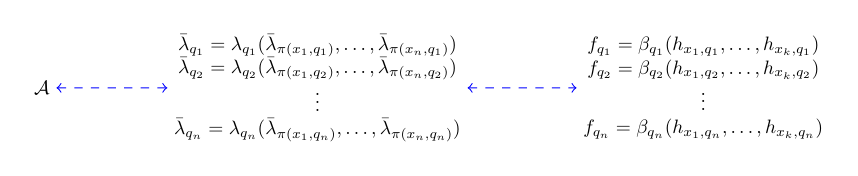
\begin{tikzpicture}[scale=0.7, every node/.style={transform shape}]
\node [align=center] (aut) at (0,-5 cm) {$\auto{A}$};
\node  [align=center,xshift=5cm] (actions) at (aut) {$\LAMBDA_{q_1}=\lambda_{q_1}(\LAMBDA_{\pi(x_1,q_1)},\ldots,\LAMBDA_{\pi(x_n,q_1)})$\\ $\LAMBDA_{q_2}=\lambda_{q_2}(\LAMBDA_{\pi(x_1,q_2)},\ldots,\LAMBDA_{\pi(x_n,q_2)})$\\ $\vdots$\\ $\LAMBDA_{q_n}=\lambda_{q_n}(\LAMBDA_{\pi(x_1,q_n)},\ldots,\LAMBDA_{\pi(x_n,q_n)})$};
\node  [align=center,xshift=12cm] (system) at (aut) {$f_{q_1}=\beta_{q_1}(h_{x_1,q_1},\ldots,h_{x_k,q_1})$\\ $f_{q_2}=\beta_{q_2}(h_{x_1,q_2},\ldots,h_{x_k,q_2})$\\ $\vdots$\\ $f_{q_n}=\beta_{q_n}(h_{x_1,q_n},\ldots,h_{x_k,q_n})$};
\draw  (aut) edge[dashed,color=blue,below,<->] node[scale=0.8,transform shape]{} (actions);
\draw  (actions) edge[dashed,color=blue,below,<->] node[scale=0.8,transform shape]{} (system);
\end{tikzpicture}
\end{figure}
\end{frame}



%\begin{frame}
%\frametitle{11. Preliminaries}
%\begin{block}{Infinite dihedral group}
%The infinite dihedral group is the semidirect product $\Z_2\ltimes_\phi\Z$ where $\phi(0)(z)=z,\phi(1)(z)=-z$. The group $\Z_2\ltimes_\phi\Z$ acts on $\Z$ from the left:
%\begin{equation*}
%(0,m)z=m+z\qquad (1,0)z=-z\qquad (1,m)=(1,0)*(0,m)
%\end{equation*}
%\end{block}
%\centering
%\begin{tikzpicture}[scale=0.65,every node/.style={transform shape}]
%\draw[latex-] (-8.5,0) -- (8.5,0) ;
%\draw[-latex] (-8.5,0) -- (8.5,0) ;
%\foreach \x in  {-7,-6,-5,-4,-3,-2,-1,0,1,2,3,4,5,6,7}
%\draw[shift={(\x,0)},color=black] (0cm,3pt) -- (0pt,-3pt) node (\x) {};
%\foreach \x in {-7,-6,-5,-4,-3,-2,-1,0,1,2,3,4,5,6,7}
%\draw[shift={(\x,0)},color=black] (0pt,0pt) -- (0pt,-3pt) node[below] 
%{$\x$};
%\end{tikzpicture}
%\pause
%\begin{block}{Lamplighter group}
%The lamplighter group is the wreath product $\Z\wr\Z_2=\Z\ltimes\Z_2^{(\Z)}$. The composition rule becomes:
%$$(\textcolor{red}{z_2},(h_i)_{i\in\Z})*(\textcolor{red}{z_1},(k_i)_{i\in\Z})=(\textcolor{red}{z_2+z_1},(h_{i+\textcolor{red}{z_1}}+_{\Z_2}k_{i})_{i\in\Z})$$
%\end{block}
%\centering
%\begin{tikzpicture}[scale=0.65,every node/.style={transform shape}]
%\draw[latex-] (-8.5,0) -- (8.5,0) ;
%\draw[-latex] (-8.5,0) -- (8.5,0) ;
%\foreach \x in  {-7,-6,-5,-4,-3,-2,-1,0,1,2,3,4,5,6,7}
%\draw[shift={(\x,0)},color=black] (0pt,0.7cm) -- (0pt,-3pt) node (\x) {};
%\foreach \x in {-7,-6,-5,-4,-3,-2,-1,0,1,2,3,4,5,6,7}
%\draw[shift={(\x,0)},color=black] (0pt,0pt) -- (0pt,-3pt) node[below] 
%{$\x$};
%\foreach \x in {-7,-4,-3,1,2,3,7}
%\filldraw[color=yellow]([yshift=0.7cm]\x) circle (0.3cm);
%\foreach \x in {-7,-6,-5,-4,-3,-2,-1,0,1,2,3,4,5,6,7}
%\filldraw[color=black]([yshift=0.7cm]\x) circle (0.1cm);
%\filldraw[color=red]([yshift=-0.7cm]-1) circle (0.2cm);
%\end{tikzpicture}
%\end{frame}



\begin{frame}
\frametitle{11. The classification theorem}
\begin{block}{Theorem}
Let $\auto{A}$ be a 2-state  automaton over the alphabet $X=\{0,1\}$ and $G$ the group defined by this  automaton. Then $G$ is isomorphic to one of the following groups:
\begin{itemize}
\item the trivial group $\{1_G\}$,
\item $\Z_2$,
\item $\Z_2\times\Z_2$,
\item $\Z$,
\item the infinite dihedral group $\Z_2\ltimes_\phi\Z$ (where $\phi(h)(z):=z(-1)^{h}$),
\item the lamplighter group $\Z\wr\Z_2=\Z\ltimes\Z_{2}^{(\Z)}$ (where $\Z$ acts on itself by $mz:=z+m$).
\end{itemize}
\end{block}
\end{frame}


\begin{frame}
\frametitle{12. Sketch of proof}
\begin{block}{Define the cases}
Let $\QQ=\{r,s\}$ and $a=\LAMBDA_r,b=\LAMBDA_s$, then 
\begin{figure}[h]
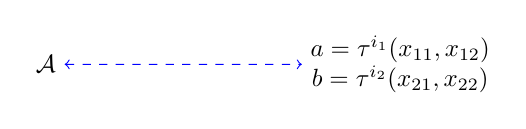
\begin{tikzpicture}[scale=0.9, every node/.style={transform shape}]
\node [align=center] (aut) at (0,-5 cm) {$\auto{A}$};
\node  [align=center,xshift=5cm] (system) at (aut) {$a=\tau^{i_1}(x_{11},x_{12})$\\ $b=\tau^{i_2}(x_{21},x_{22})$};
\draw  (aut) edge[dashed,color=blue,below,<->] node[scale=0.8,transform shape]{} (system);
\end{tikzpicture}
\end{figure}
where $x_{ij}\in\{a,b\}$ and $\tau^{i_1},\tau^{i_2}\in\symm(\abece)=\symm(\{0,1\})$. There are 64 possibilities. We proceed by analyzing a part of them.
\end{block}
%\pause
%\begin{block}{Case analysis}
%Let $\tau$ be the transposition of $\symm(\abece)$. Every case is analogous to one of the 24 cases where $a\in\{\tau(a,a),\tau(a,b),\tau(b,b)\}$. We proceed by analysing part of them.
%\end{block}
\end{frame}


%\begin{frame}
%\frametitle{Conclusion}
%\begin{figure}[ht]
%\begin{tikzpicture}
%\node[state] (a) at (0,0) {$a,\sigma$};
%\node[state, right of=a, xshift=60] (b) {$b, 1$};
%\draw	(a) edge[left, loop left, ->] node{$1$} (a)
%		(a) edge[bend left,->, above] node{$0$} (b)
%		(b) edge[loop right, ->, right] node{$0$} (b)
%		(b) edge[below, bend left,->] node{$1$} (a);
%		
%\end{tikzpicture}
%\caption{Automaton which defines the Lamplighter group}
%\end{figure}
%\end{frame}





\begin{frame}
\begin{Huge}
Thank you for your attention!
\end{Huge}
\end{frame}

%\begin{frame}
%\frametitle{The Lamplighter Group*}
%\begin{block}{Ingvioletients}
%\begin{itemize}
%\item Direct sum of $\Z_2$ on $\Z$:
%$${\Z_2}^{(\Z)}=\bigoplus_{j\in\Z} {\Z_2}^{j}:=\{(b_j)_{j\in \Z}| b \in \Z^2, b_j\neq 0\textrm{ for a finite number of j}\}$$
%\item Action through Translation of $\Z$ on $\Z_2$:
%$$\phi:\Z\times{\Z_2}^{(\Z)}\longrightarrow\Z_2$$ $$\phi(z,(b_j)_{j\in\Z}):=(b_j)_{j-z\in\Z}$$
%\end{itemize}
%\end{block}
%\begin{block}{Definition of $\Z\wr\Z_2$}
%The Lamplighter group is the set $\Z\times{\Z_2}^{(\Z)}$ provided with the operation:
%$$(z_1,({b^1}_j)_{j\in\Z})*(z_2,({b^2}_j)_{j\in\Z}):=(z_1 +z_2,({b^1}_j+{b^2}_{j-z_1})_{j\in\Z})$$
%\end{block}
%\end{frame}


\end{document}